\chapter{A data-driven background estimate}
We identified three sources of backgrounds
(page~\pageref{page:background_categories}). The backgrounds from charge
misidentification and from non-prompt leptons are analysed with data driven
techniques.
\section{Charge misidentification}
Standard Model processes with prompt leptons of opposite charge are very
common at the LHC. They can contribute to the top partners background if the
charge of one of the leptons is incorrectly measured.
For muons in the \pt range considered in this analysis, the charge misidenfication rate is extremely small ($10^{-4}-10^{-5}$) and their contribution to the background is
negligible~\cite{susy2011}. The magnitude of this contribution due to electrons can be derived from the data by using the \Z boson resonance. 
The fraction of misidentified leptons is obtained by considering events with two electrons in which the invariant mass of the leptons falls inside the 
\Z boson mass window: $\unit[76]{GeV}< M(\Lep \Lep) <\unit[106]{GeV}$. These events must pass all cleaning and trigger requirements and the electrons are likewise required to pass all 
quality cuts, but the selection based on the number of jets. As can be seen in the tables~\ref{tab:ZWindowBkgd} and~\ref{tab:ZWindowSig}, this sample is expected to be completely dominated by $\Z$+jets.

\begin{table}[htb]
    \centering
\begin{tabular}{*9c}
    \toprule
                & total & \ttbar    & $\Z$+jets & $\W$+jets & $\W\Z$ & $\Z\Z$ & \ttbar$\W$ & \ttbar$\Z$   \\
                \midrule
                In $\Z$-window & 9.3$\cdot 10^{5}$      & 644       & 9.3$\cdot 10^{5}$      &  35        & 205   &  46.2   & 1.89      & 8.62      \\
 same-sign      & 1090         & 1.84      & 1050       & 9.97      & 8.9   &  1.02   & 0.62      & 0.20      \\
 \bottomrule
\end{tabular}
\caption{Expected event yields within the \Z invariant mass window ($\unit[76]{GeV}< M(\Lep \Lep) <\unit[106]{GeV}$) for the background contributions. The backgrounds not shown yield negligible
         contributions to this phase space region.}
\label{tab:ZWindowBkgd}
\end{table}

\begin{table}[htb]
    \centering
\begin{tabular}{*9c}
    \toprule
$T_{5/3}$ mass [GeV]  & 400       & 450       & 500       & 550       & 600       & 650       & 700       & 750       \\ 
\midrule
 in \Z window         & 22.6      & 9.84      & 4.04      & 1.81      & 0.928     & 0.464     & 0.224     & 0.123     \\ 
 same-sign           & 12.1      & 4.74      & 1.79      & 0.716     & 0.359     & 0.145     & 0.075     & 0.0345    \\ 
 \bottomrule
\end{tabular}
\caption{Expected event yields within the \Z invariant mass window
    ($\unit[76]{GeV}< M(\Lep \Lep) <\unit[106]{GeV}$) for the eight \TP signal  points.}
\label{tab:ZWindowSig}
\end{table}


Applying the same method to data we obtain $858330$ events in the \Z mass
window; $1014$ events remain upon applying the same-sign requirement. The probability of misidentifying the charge of each 
lepton is computed by assuming that the entirety of the same-sign contribution is due to misidentified \Z+jets events and is found to be $5.89 \times 10^{-4}$. To confirm that this upper limit is close to the true probability, we consider the dilepton invariant mass spectrum shown in Figure~\ref{fig:ZWindowMassPeak}. Both 
the simulation and the mass spectrum suggest that the upper limit is close
to the true probability (within approximately 1\% according to the
simulation). We note that this  estimated charge misidentification
probability is consistent with the measurement in~\cite{susy2011}.

\begin{figure}[htb]
\centering
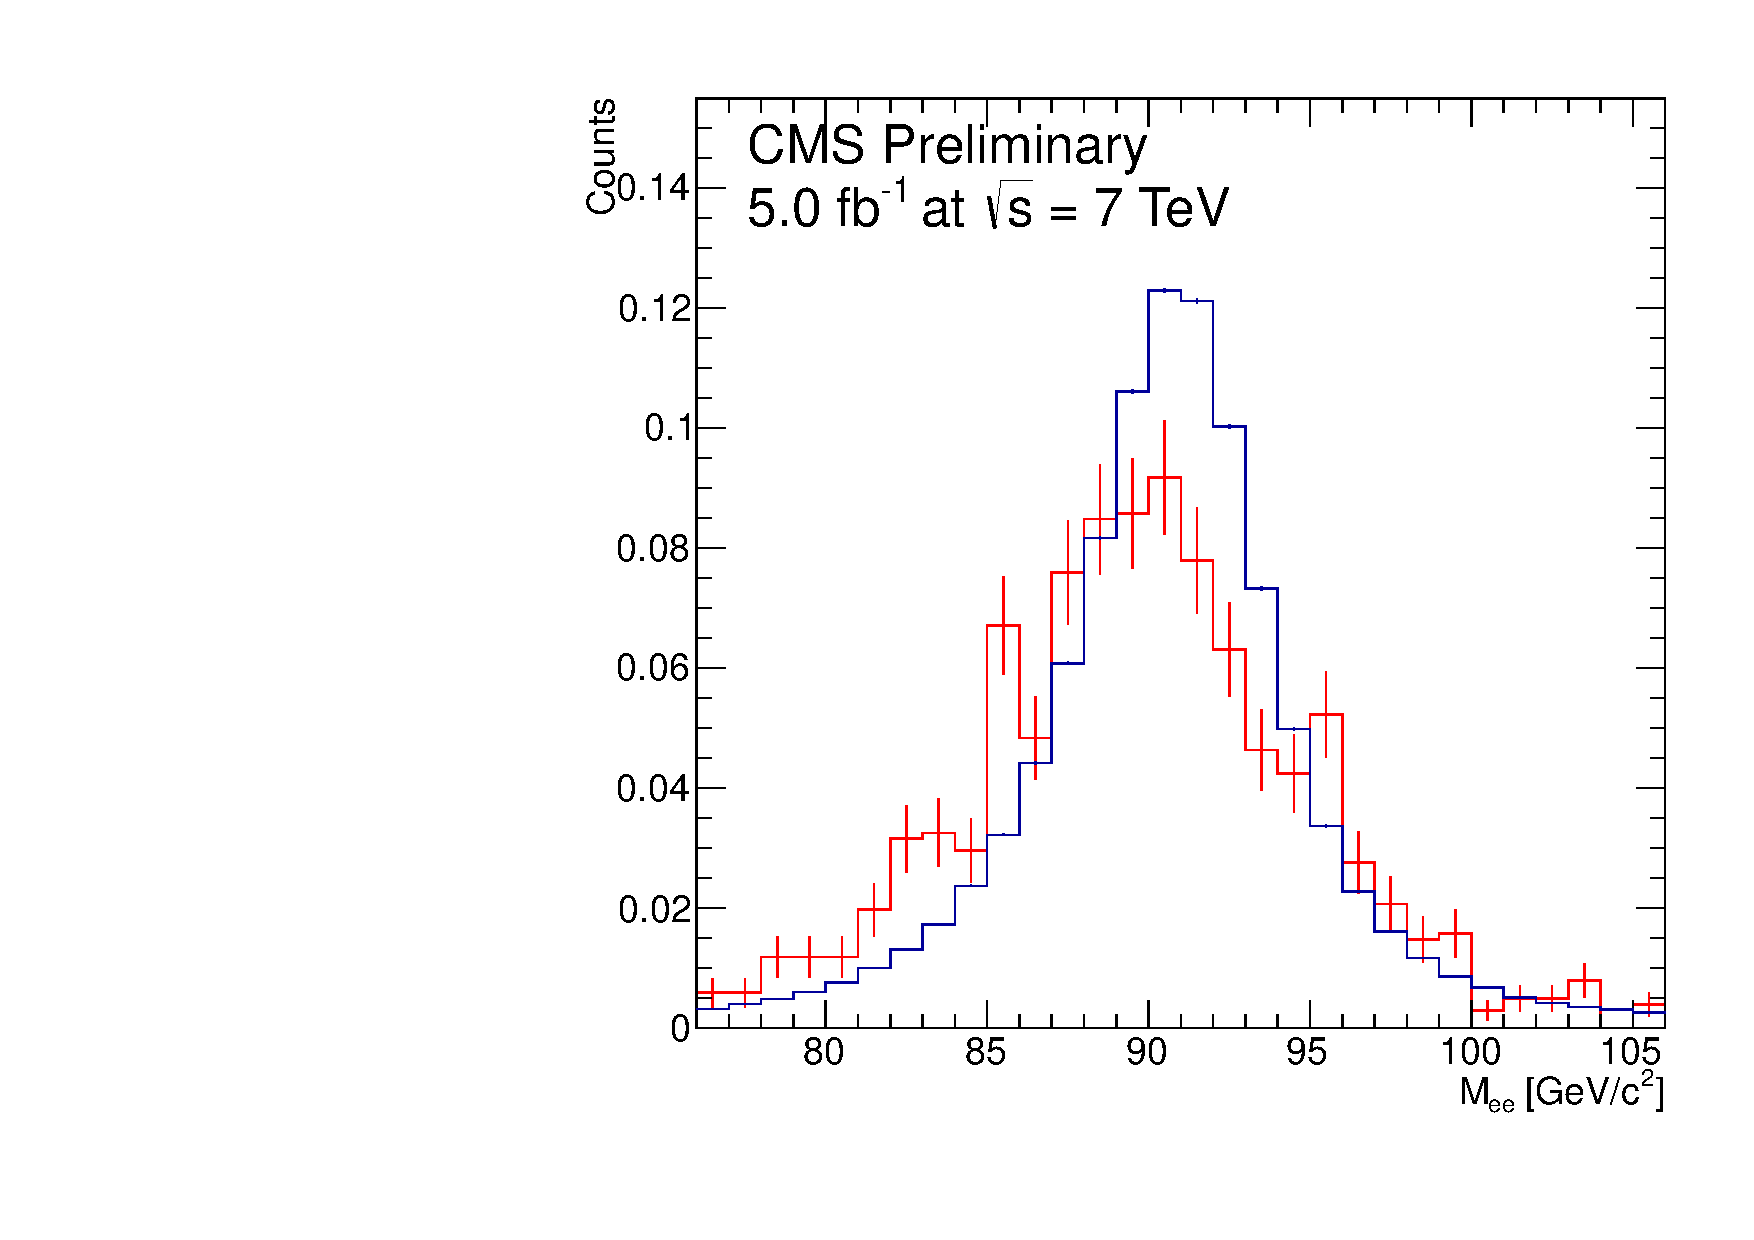
\includegraphics[width=\textwidth]{images/pdf/ChargeMisID_ZMass.pdf}
\caption{The dilepton invariant mass spectrum for electrons in data. The opposite-sign distributions are shown in blue and 
the same-sign ones are in red. Both distributions are normalized to unit area.}
\label{fig:ZWindowMassPeak}
\end{figure}

The distributions of the charge misidentification probability as a function of \pt and $\eta$ are shown in Figure~\ref{fig:ChargeMisIDprob}.
The probability is essentially flat as a function of \pt up to the point where statistical uncertainties become large. The $\eta$ distribution
shows that the charge of central electrons is much less likely to be misidentified than the charge of electrons in the endcaps.

\begin{figure}[tbp]
\begin{center}
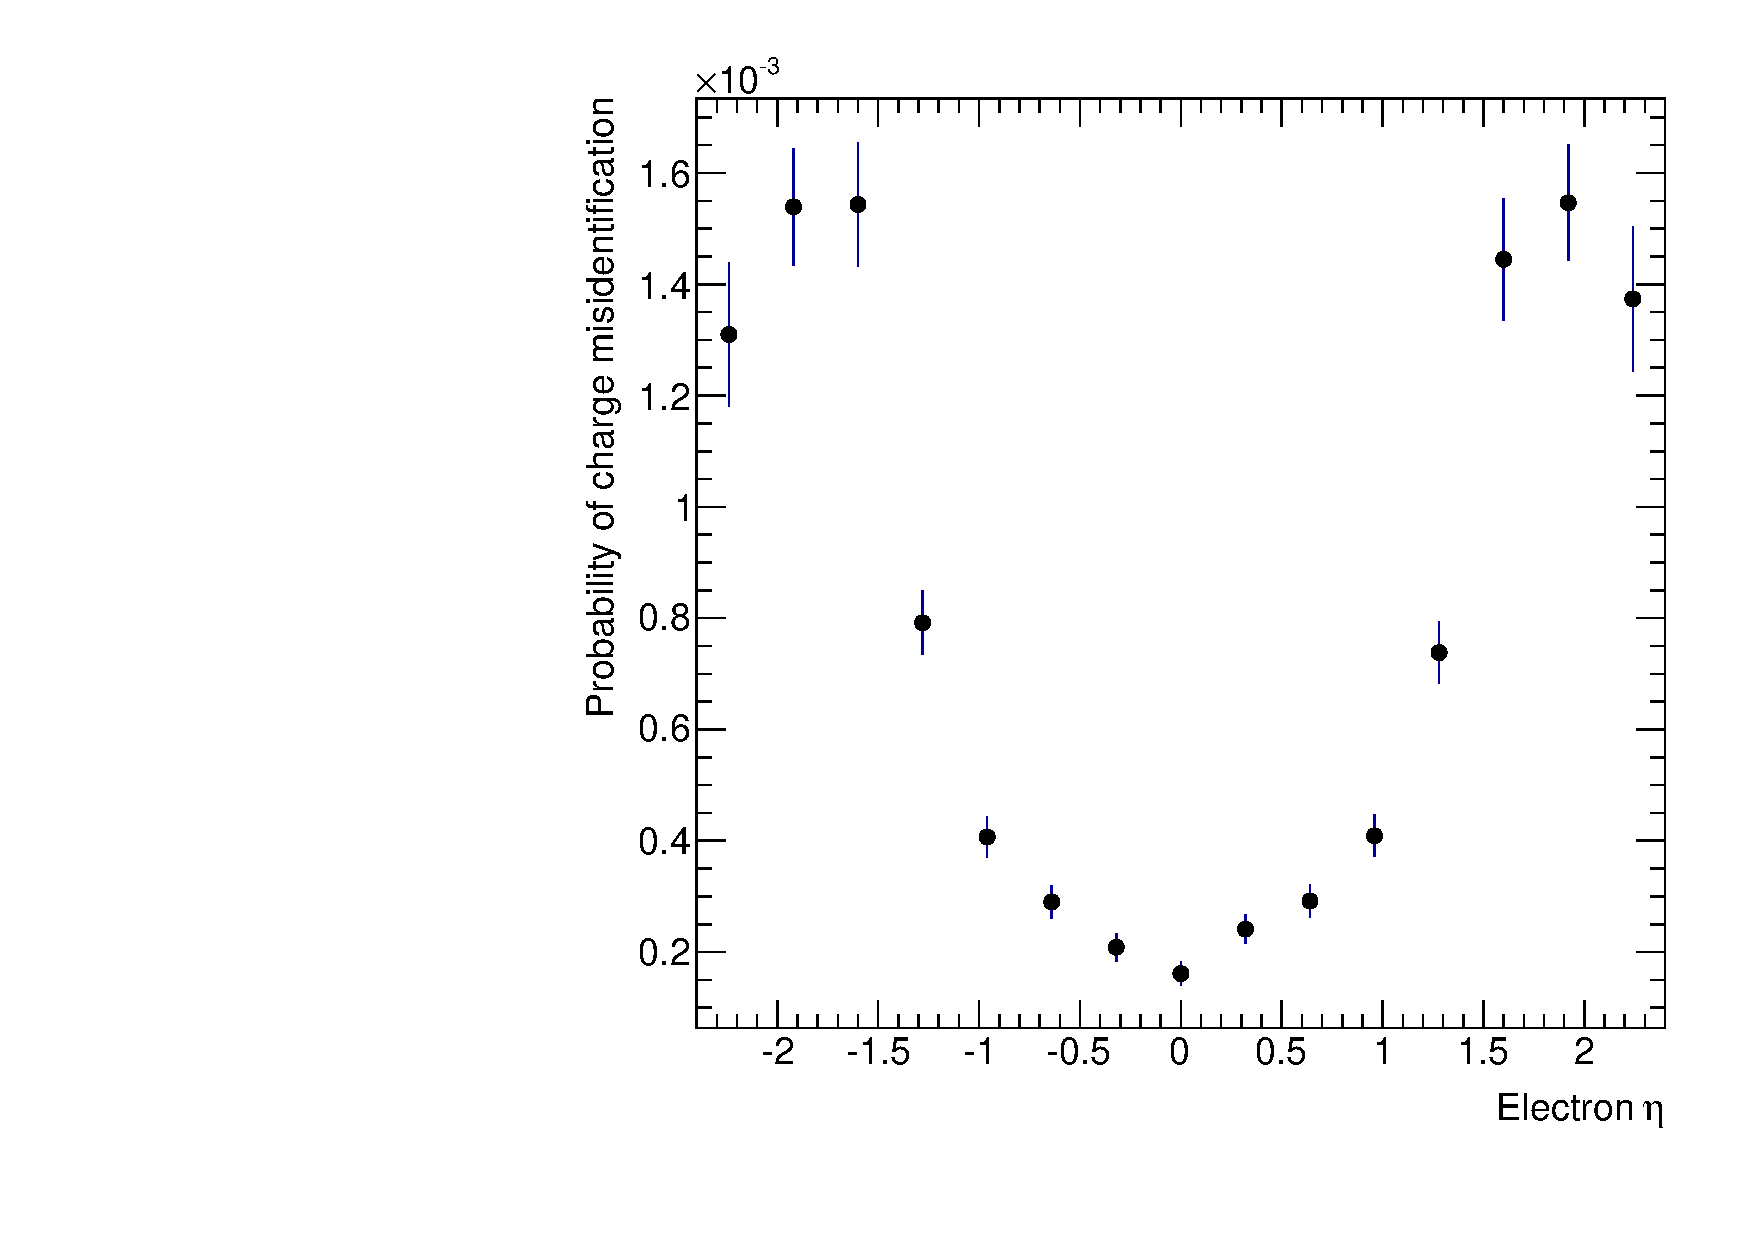
\includegraphics[width=0.49\textwidth]{figures/h_MisIDProbvsEta.pdf} \hfill
\includegraphics[width=0.49\textwidth]{figures/h_MisIDProbvsPt.pdf} \\ 
\caption{The distributions of the electron charge misidentification probability as a function of $\eta$ (left) and \pt (right).}
\label{fig:ChargeMisIDprob}
\end{center}
\end{figure}

The number of expected same-sign events due to charge misidentification is estimated by considering the total number of events passing the 
full selection (including the jet and $H_{T}$ requirements as well as the $\Z$-veto), but having oppositely charged leptons. These events are weighted by
the charge misidentification probability parametrized as a function of eta. The results are shown in Table~\ref{tab:ChargeMisIDResult}. 
In addition, we assign a systematic uncertainty of 20\% based on the variation between results obtained using the average probability and the $\eta$-dependent one. 

\begin{table}[!htbp]
    \centering
\begin{tabular}{ccc}
\hline \hline
       & Opposite-sign & Expected same-sign \\
\hline 
$\E\E$   & 171           & 0.18  $\pm$ 0.04  \\
$\E\M$   & 308           & 0.14  $\pm$ 0.03  \\
\hline \hline
\end{tabular}
\caption{The numbers of opposite sign events passing the full selection and the expected contribution of same-sign events due to charge misidenfication.}
\label{tab:ChargeMisIDResult}
\end{table} 
